\documentclass{article} % COLM 2026 template (official kit, tag 2026)
\usepackage[submission]{colm2026_conference}

\usepackage{microtype}
\usepackage{hyperref}
\usepackage{url}
\usepackage{booktabs}
\usepackage{enumitem}
\usepackage{amsmath}
\usepackage{graphicx}
\usepackage{lineno}

\definecolor{darkblue}{rgb}{0, 0, 0.5}
\hypersetup{colorlinks=true, citecolor=darkblue, linkcolor=darkblue, urlcolor=darkblue}

\title{Three Bounds on a Null: Testing the Link Between Fast-Weight Write
Geometry and In-Context Composition}

% Anonymized for double-blind review; the submission option suppresses this
% block regardless.
\author{Anonymous authors}

\begin{document}

\ifcolmsubmission
\linenumbers
\fi

\maketitle

\begin{abstract}
Fixed-state sequence models bind in-context associations in a matrix-valued
fast-weight state, and geometric observables of that state, such as the span
occupied by key writes, have been proposed as lenses on composition. We test
whether one such observable predicts, or causally improves,
in-context multi-hop composition in DeltaNet-family language models spanning
14M to 1.31B parameters, and we find a null bounded three ways. First, a
state-space composition readout returns a recovered fraction of exactly zero
at 366 of 366 readings % evidence: C1-phase1
across three structurally different instruments (zero-shot marker prompts,
natural language, and task-familiarized checkpoints); the readout's
pre-registered validity gates fail at every cell, so the zeros are an
instrument verdict, not a refutation. Second, a
vocabulary-space behavioral contrast bounds any causal effect of a
write-geometry intervention below its pre-registered three-seed detection
floor of 1.5 to 1.7 loss units; % evidence: C5-power
the sole reading meeting the pre-registered differential condition (one of
five that exclude zero across forty tests) is a transient, harm-direction
deviation. Third, a twelve-seed replication of the transient was
stopped by its pre-registered batch-effect gate (cohort variance ratio
4.47 against a heuristic cutoff of 4.0), % evidence: C7-replication
and the new cohort's interval spans zero. Each bound names the observation
that would overturn it. The result is a null with its assumptions visible
and its escape routes closed.
\end{abstract}

\section{Introduction}

Linear-attention and delta-rule language models compress an entire context
into a fixed-size matrix state
\citep{schlag2021linear,yang2024parallelizing}. A companion research program
measured \emph{geometric} observables of the written state (the span
fraction occupied by key writes, the effective rank of the key population)
across scales and under targeted interventions, carrying an unexamined
promise: that write geometry matters for something a user would recognize,
such as composing multi-hop relations presented in context. We test that
promise and find a null. A reader of a null has two standing worries, that
the instrument never worked and that the analysis could declare a null
after seeing the data. Three pre-registered bounds address both:

\begin{enumerate}[leftmargin=1.5em,itemsep=1pt,topsep=2pt]
\item \textbf{An instrument bound.} A state-space composition readout,
deployed three structurally different ways, returns a recovered fraction of
exactly zero at 366 of 366 readings % evidence: C1-phase1
on checkpoints from 14M to 1.31B parameters, and its pre-registered
validity gates fail at every cell, routing the outcome to probe-invalid,
not refutation. One nonzero reading or one gate pass would have voided
this bound.
\item \textbf{A power bound.} A vocabulary-space behavioral contrast, with
a three-seed detection floor of 1.5 to 1.7 loss units registered before
unblinding, % evidence: C5-power
leaves three of the four per-arm contrasts unresolved; the sole reading meeting the
pre-registered differential condition is a transient, harm-direction
deviation. % evidence: C6-transient
A determinate effect above the floor would have voided this bound.
\item \textbf{A replication bound.} A targeted twelve-seed extension of
that transient was stopped by its own pre-registered batch-effect gate
(a 4.47-fold cohort variance mismatch against a heuristic 4.0 cutoff),
% evidence: C7-replication
and the new cohort's interval spans zero. A clean pooled interval excluding
zero would have voided this bound.
\end{enumerate}

The contribution is the bounded null and the measurement discipline that
kept it interpretable.

\section{Models, Task, and Instruments}
\label{sec:setting}

\textbf{Checkpoints and task.} All experiments probe DeltaNet-family
language models \citep{yang2024parallelizing} pretrained on a
reasoning-dense corpus mix (OpenR1-Math) and an encyclopedic mix
(WikiText-103, \citealp{merity2017pointer}). An \emph{intervention grid}
(14M parameters) varies a frozen-key-bias intervention on the fast-weight
write path in three validation-loss-matched arms: control, per-token, and
global. A \emph{scale ladder} spans 14M, 98M, 392M, and 1.31B parameters
(state dimension 64, 64, 128, 128; depth 2, 12, 16, 22).
% evidence: C0-ladder
Each probe episode binds $K$ entities into one directed cycle with
\textsc{bind} statements, then queries the entity $h \in \{1,\dots,4\}$
hops around the cycle; a full $K$-cycle prevents held-out hop depths from
collapsing modulo short cycle lengths. Load is $K$ relative to state
dimension ($K \in \{20, 32\}$ on the grid; near-capacity per rung).

\textbf{Instrument 1: a geometric readout.} For a layer's terminal state
$S_T$ and effective query $q_{\mathrm{eff}}$, the readout predicts the
$h$-hop target as $S_T^{\,h} q_{\mathrm{eff}}$ and scores \emph{exact
continuous recovery}: the fraction of queries reaching cosine at least 0.9
with the target value vector. Continuous recovery, rather than argmax over
candidates, follows \citet{nichani2024understanding}, under which argmax
decoding can succeed without the state carrying the claimed structure.
Registered validity gates accompany the readout: an $h{=}1$ sanity floor
and two alignment premises, (iii) query--key and (iv) key--value, each
requiring a same-entity median cosine above a shuffled-entity null's 95th
percentile (Appendix~\ref{app:gates}); gate failure routes to
probe-invalid, never to refutation.

\textbf{Instrument 2: a behavioral contrast.} A familiarization phase
trains checkpoints for 5{,}000 steps on the bind/query task mixed into the
pretraining corpus; the contrast is the held-out-episode query loss $L_q$
(a vocabulary-space cross-entropy through the language-model head,
machinery disjoint from Instrument 1), differenced control minus arm at
five checkpoints. A six-outcome trajectory classification and a
differential condition (the $K{=}32$ effect determinate while $K{=}20$ is
not) were fixed before unblinding. Every wave ran gate-first, with
verdicts routed mechanically (Appendix~\ref{app:gates}).

\section{The Geometric Readout Never Fires}
\label{sec:geometric}

\begin{table}[t]
\centering
\footnotesize
\setlength{\tabcolsep}{3.5pt}
\begin{tabular}{@{}llll@{}}
\toprule
Wave (instrument) & Grid & Readings & Registered outcome \\
\midrule
1 zero-shot, marker & 78 cells, 14M--392M & 312/312 $= 0.0$ & probe-invalid \\ % evidence: C1-phase1
2 zero-shot, 1.31B rung & 2 cells & 8/8 $= 0.0$ & probe-invalid \\ % evidence: C2-rung3
3 zero-shot, natural lang. & 4 gate cells & 16/16 $= 0.0$ & probe-invalid, refused \\ % evidence: C3-phase1b
4 familiarized gate & 6 cells $\times$ 5 ckpts & 30/30 $= 0.0$; $L_q$ falls & dissociation \\ % evidence: C4-dissoc
5 behavioral contrast & 18 cells, 4 contrasts$^{\dagger}$ & 3 unresolved, 1 transient & power-bounded \\ % evidence: C5-power
6 seed extension, $n{=}12$ & 18 pretrain cells & variance ratio 4.47 & batch-effect-flagged \\ % evidence: C7-replication
\bottomrule
\end{tabular}
\caption{The program at a glance. Waves 1--4 deploy the geometric readout
(recovered fraction at cosine $\geq 0.9$); its validity gates fail at every
cell of every wave, so all zero readings route to probe-invalid rather than
refutation. Waves 5--6 deploy the vocabulary-space contrast; the one
determinate transient is in the harm direction and its $n{=}12$ replication
was stopped by the pre-registered batch-effect gate.
$^{\dagger}$Per-arm re-derivation; the registered corpus-level pipeline
returned both corpora unresolved (Appendix~\ref{app:gates}).}
\label{tab:program}
\end{table}

\textbf{Zero-shot, marker template (wave 1).} The full pre-registered
grid, 60 intervention cells and 18 ladder cells
(Table~\ref{tab:program}), returns a recovered fraction of exactly 0.0 at
all 312 (cell, hop) readings. % evidence: C1-phase1
The validity gates fail everywhere: the $h{=}1$ floor fails both
conditions, and premises (iii) and (iv) pass at 0 of 78 cells each.
% evidence: C1-phase1
Premise medians track their shuffled nulls but never cross them (premise
(iii) spans $[-0.33, 0.76]$), % evidence: C1-phase1
and prediction--target cosines center near zero, ten-plus standard
deviations from the 0.9 threshold (Figure~\ref{fig:gates},
Appendix~\ref{app:figs}).

\textbf{Scale (wave 2).} The 1.31B rung reproduces the failure in kind:
8 of 8 readings at 0.0, both premise gates failing at both corpora, for a
ladder series of 80 of 80 zeros across 14M to 1.31B:
% evidence: C2-rung3
not a small-model artifact.

\textbf{Zero-shot, natural language (wave 3).} Two template families, a
gift-verb family with the out-of-distribution query marker dropped and a
corpus-native succession-verb family, fail identically: 16 of 16 readings
at 0.0, the $h{=}1$ gate false at all 4 cells. % evidence: C3-phase1b
The failure is not attributable to prompt surface form.

\textbf{Task-familiarized (wave 4).} The strongest-case test trains
control checkpoints on the task itself for 5{,}000 steps and applies the
gate at five checkpoints per cell. It fails at 30 of 30 readings, 0 of 512
queries recovered each time, % evidence: C4-dissoc
while the vocabulary-space query loss falls 21.8 to 46.4 percent (mean
35.9 percent) in 6 of 6 cells, measured from checkpoint 250, the first
post-warmup reading, to checkpoint 5{,}000 % evidence: C4-dissoc
(Figure~\ref{fig:dissoc}, Appendix~\ref{app:figs}): the models measurably
learn the task through one readout while the other stays at floor. Since
the two share no machinery by construction, the dissociation indicts the
readout construct, not the models (the fall stops short of a registered
50-percent pin, so the adjudication claims partial task learning only).

\textbf{Gates with enforcing code paths.} Wave 1's launch chain computed
its abort gate but had no code path acting on it; the grid ran past a gate
that had already declared the probe invalid. % evidence: C8-teeth
Every later chain enforced its gates at the process boundary; waves 3 and
4 each refused a full-grid launch on a real failing gate.
% evidence: C8-teeth

\section{The Behavioral Contrast Is Power-Bounded}
\label{sec:behavioral}

Wave 5 promotes the vocabulary-space contrast to the primary instrument:
all three arms are familiarized under identical recipes (18 cells), and
the arm effect is the held-out query-loss difference, control minus arm,
so positive means the intervention helps.

\textbf{The registered power floor.} Before unblinding, the three-seed
detection floor was derived from the control cells' between-seed spread: a
$\sigma$ proxy of 0.43 to 0.48 loss units gives a 95-percent half-width of
roughly 1.5 to 1.7. % evidence: C5-power
For calibration, the entire familiarization effect is about 1.69 loss
units: % evidence: C5-power
the instrument detects only effects about as large as everything the model
learns in the phase, so the registration anticipated unresolved outcomes,
to be read as measurement bounds, never as evidence of no effect.

\textbf{Results.} The registered corpus-level classifier, which uses the
global arm as each corpus's representative, returns both corpora
unresolved; a disclosed build-time per-arm re-derivation (folded into the
analysis code, re-validated against the archived deltas;
Appendix~\ref{app:gates}) splits this into four contrasts, three
unresolved. % evidence: C5-power
The fourth (encyclopedic corpus, per-token arm) classifies as transient:
at checkpoint 2{,}500 the $K{=}32$ effect is determinate at $-0.500$,
interval $[-0.624, -0.376]$, while $K{=}20$ is not, and by checkpoint
5{,}000 it dissolves
% evidence: C6-transient
(Figure~\ref{fig:transient}, left, Appendix~\ref{app:figs}). A
held-out-hop secondary readout fires at the same cell and checkpoint, same
direction, % evidence: C6-transient
consistent with one coherent mid-training deviation.

\textbf{Sign discipline and multiplicity.} Of 40 uncorrected 95-percent
intervals in the primary table, five exclude zero against two expected by
chance, all in the harm direction (arm loss above control); four of the
five sit at checkpoint 1{,}000, both loads of two different cells,
consistent with checkpoint-level sampling noise (Appendix~\ref{app:gates}).
Only the fifth, at checkpoint 2{,}500, also satisfies the pre-registered
differential condition and draws the held-out-hop corroboration; that
compound condition, not any single interval, is the one determinate signal.
% evidence: C6-transient
``The intervention matters'' ignores that transients were registered as
training-dynamics artifacts; ``no effect'' ignores the power floor.

\section{The Replication Gate Refuses the Pool}
\label{sec:replication}

Wave 6 extends the transient's anchor cell (encyclopedic corpus, per-token
arm, $K{=}32$, checkpoint 2{,}500) to twelve seeds with three registered
integrity mechanisms: nine fresh pretraining seeds per arm (18 cells), an
archived-values loader whose runtime guard forbids live re-scoring,
% evidence: C7-replication
and a pre-pooling batch-effect gate (means within twice the pooled
standard error; variance ratio below 4.0).

\textbf{The gate fired.} The archived cohort's between-seed standard
deviation (1.154) is 2.1 times the new cohort's (0.546): variance ratio
4.47, past the heuristic 4.0 cutoff (a routing threshold, not a calibrated
test; the one-sided 5-percent $F(2,8)$ value is ${\approx}4.46$); the
means agree (shift 0.364, threshold 1.382). % evidence: C7-replication
The registered routing reports the cohorts separately, batch-effect-flagged,
with no decision-grade pooled interval: the archived cohort reproduces its
original $[-0.624, -0.376]$ by construction; the new nine-seed cohort's own
interval, $[-0.506, +0.357]$, spans zero; % evidence: C7-replication
and the naive twelve-seed pool, diagnostic only, reads $[-0.509, +0.147]$,
a refutation absent the gate % evidence: C7-replication
(Figure~\ref{fig:transient}, right, Appendix~\ref{app:figs}).

\textbf{What stands.} The transient is neither confirmed nor refuted; it
keeps its three-seed weight. Every computable pooled interval, at 7 of 10
primary and 7 of 10 held-out (checkpoint, load) pairs, contains zero.
% evidence: C7-replication
The variance mismatch is not established as systematic; its direction
flips across checkpoints, consistent with small-$n$ imprecision in the
archived cohort.

\section{Related Work}
\label{sec:related}

Zoology \citep{arora2023zoology} and Based \citep{arora2024simple}
establish the recall--state-size tradeoff and the ladder pattern this
program follows; both train architectures for the probe setting, where
this program probes general-purpose checkpoints post hoc and reports
instrument validity, not a capacity frontier.
\citet{okpekpe2025revisiting} show that optimizer choice, not architecture
alone, drives much of the reported Transformer--recurrent recall gap; this
paper bounds a different axis, write-geometry validity, and makes no
positive mechanism claim. \citet{grazzi2024unlocking} prove
positive-eigenvalue DeltaNet cannot compose certain groups (e.g.\ parity),
a ceiling lifted only by negative-eigenvalue transitions;
\citet{merrill2024illusion} give the analogous $\mathrm{TC}^0$ ceiling for
diagonal SSMs.
\citet{nichani2024understanding} supply the associative-memory analysis
behind the exact-recovery readout (Section~\ref{sec:setting}). Reporting
follows the pre-registration workshop \citep{bertinetto2021preface} and
negative-results tradition \citep{forde2020icbinb}.

\section{Scope of the Bounds}
\label{sec:scope}

\textbf{Bounded.} The readout construct, one layer's terminal state
applied $h$ times to a query under exact continuous recovery, carries no
signal in this checkpoint family at any tested scale, surface form, or
training regime. % evidence: C4-dissoc
Intervention effects beyond 1.5 to 1.7 loss units either way are excluded
at the registered confidence; % evidence: C5-power
the transient is bounded in duration, direction, and weight.
% evidence: C7-replication

\textbf{Not bounded.} The hypothesis survives below the power floor and
through mechanisms the readout cannot see, most plausibly cross-layer
hand-off (one layer resolves the first hop, a later layer the next); the
readout tests only single-layer self-iteration. A competing account is
expressivity: \citet{grazzi2024unlocking} prove positive-eigenvalue
DeltaNet cannot compose certain permutation groups, so the null may
partly reflect this variant's ceiling rather than a wrong observable;
wave 4's dissociation points toward the observable; and nothing here
transfers beyond the DeltaNet family or the bind/query grammar. Finally,
the readout's recovery math is validated only at unit level, never
end-to-end on a real forward pass with a known target, so a systematic
extraction or state-convention error is not fully excluded
(Appendix~\ref{app:gates}); a real-kernel positive control is the next
wave's priority.

\textbf{Lessons for small-scale practice.} A registered gate without an
enforcing code path is a sentence, not a safeguard (refusal worked twice
on real failures); % evidence: C8-teeth
routing fixed before unblinding kept zeros from becoming a refutation and
a transient from becoming a headline.


\bibliography{refs}
\bibliographystyle{colm2026_conference}

\appendix

\section{Registered Gates and Routing Rules}
\label{app:gates}

This appendix reproduces, in compact form, the pre-registered gates and
mechanical routing rules the main text relies on. Each was fixed in the
program's design registry before the corresponding data existed.

\textbf{Geometric-readout validity gates (waves 1--4).} A cell's readout is
valid only if all of the following hold. (a) \emph{$h{=}1$ sanity floor:}
the one-hop recovered fraction must exceed the upper edge of a
shuffled-pairing null by more than the null's width, and must also exceed
an absolute floor of 0.10. (b) \emph{Premise (iii):} the median cosine
between an entity's query projection and the same entity's key projection
must exceed the 95th percentile of a shuffled-entity null. (c)
\emph{Premise (iv):} the median cosine between the key and value
projections of the same token must exceed the same null percentile.
\emph{Routing:} failure of any gate routes the cell to probe-invalid; the
registered rule states that gate failure never routes to refutation.
The readout's recovery math (state-power application and the
cosine-recovery scorer) is unit-tested against hand-built matrices; it has
no positive control run end-to-end through a real forward pass with a
known target on the production multi-layer kernel path. The failure's
uniformity across four structurally different instruments and four scales
is consistent with a genuine construct-validity gap but does not, on its
own, rule out a systematic extraction or state-convention error producing
the same uniform pattern.

\textbf{Behavioral-contrast classification (wave 5).} The per-checkpoint
arm effect is $\Delta(c) = L_q(\text{control}, c) - L_q(\text{arm}, c)$,
with three-seed 95-percent intervals ($t(2, .975) = 4.303$). % evidence: C5-power
A checkpoint
satisfies the differential condition when the $K{=}32$ interval excludes
zero, the $K{=}20$ interval does not, and $|\Delta_{32}| > |\Delta_{20}|$.
Trajectories classify into six registered outcomes: persistent, transient
(the condition holds at an interior checkpoint and fails at the terminal
one), late-emergent, converged-equivalent, unresolved, and a
familiarization-null exclusion. The three-seed power floor (a detectable
effect of roughly 1.5 to 1.7 loss units, derived from the control cells'
between-seed spread) was registered together with the instruction that
unresolved outcomes be reported as measurement bounds. % evidence: C5-power

The registered pipeline computed one classification per corpus, using the
global arm as that corpus's representative signal, and classified both
corpora unresolved. % evidence: C5-power
The four-way (corpus, arm) breakdown reported in the
main text and Table~\ref{tab:program} applies the same registered
classification primitives to each arm's own trajectory. This finer split
was a build-time re-derivation performed after the corpus-level output was
seen; it was later folded into the analysis code and re-validated against
the archived per-cell deltas, reproducing the same four verdicts. It is
disclosed here as a re-derivation, not presented as the registered
corpus-level verdict.

The primary table computes 40 uncorrected 95-percent intervals (4
contrasts $\times$ 5 checkpoints $\times$ 2 loads); five exclude zero:
both loads of reasoning-dense$\times$global at checkpoint 1{,}000
($K{=}32$: $\Delta{=}{-}0.203$, $[-0.402,-0.004]$; $K{=}20$:
$\Delta{=}{-}0.199$, $[-0.325,-0.074]$), both loads of
encyclopedic$\times$per-token at checkpoint 1{,}000 ($K{=}32$:
$\Delta{=}{-}0.168$, $[-0.301,-0.036]$; $K{=}20$: $\Delta{=}{-}0.109$,
$[-0.211,-0.006]$), and the $K{=}32$ interval of
encyclopedic$\times$per-token at checkpoint 2{,}500 ($\Delta{=}{-}0.500$,
$[-0.624,-0.376]$, the reported transient). % evidence: C6-transient
Only the last also satisfies
the compound differential condition above and is corroborated by the
independent held-out-hop readout at the same cell and checkpoint; that
compound condition, not any single interval exclusion, is what the main
text calls the one determinate signal. The checkpoint-1{,}000 cells fail
the differential condition precisely because their $K{=}20$ intervals
also exclude zero.

\textbf{Replication integrity gates (wave 6).} Archived seeds load from
stored values only; a runtime guard raises on any live re-scoring of an
archived seed. Before pooling, a batch-effect gate requires (a) cohort
mean shift below twice the pooled standard error (Welch form) and (b)
cohort variance ratio below a pre-registered heuristic 4.0 (not a
calibrated $F$-test; the one-sided 5-percent $F(2,8)$ critical value for
the archived three-seed versus new nine-seed cohorts is $\approx 4.46$).
% evidence: C7-replication
On gate failure the registered
routing reports both cohorts separately, produces no decision-grade pooled
interval, and classifies the wave as batch-effect-flagged, outside the
four-outcome partition (confirmed at magnitude, confirmed smaller,
refuted, new pattern) that a passing gate would have entered.

\clearpage
\section{Supplementary Figures}
\label{app:figs}

\begin{figure}[h]
\centering
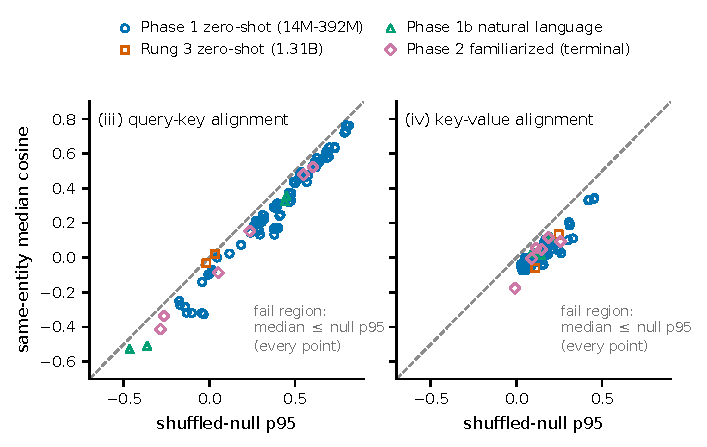
\includegraphics[width=0.92\linewidth]{figures/fig1_validity_gates.pdf}
\caption{Validity-gate failure at every cell of every instrument. Each
point is one cell's same-entity median cosine for premise (iii)
(query--key, left) or premise (iv) (key--value, right) against that cell's
shuffled-entity null p95; passing requires a median above the dashed
identity line. All 90 cells across the four geometric-readout waves fall
on or below the line, at every scale from 14M to 1.31B and under every
surface form and training regime.}
% evidence: C1-phase1, C2-rung3, C3-phase1b, C4-dissoc
\label{fig:gates}
\end{figure}

\begin{figure}[h]
\centering
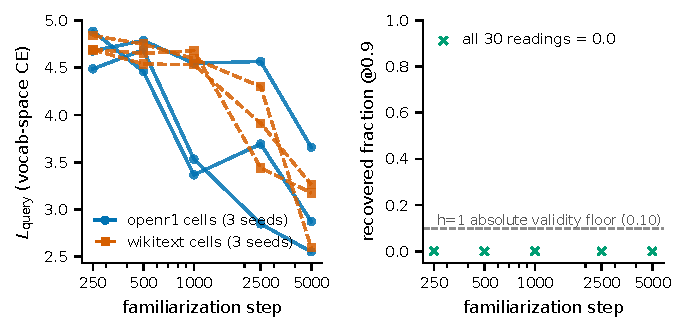
\includegraphics[width=0.92\linewidth]{figures/fig2_dissociation.pdf}
\caption{Vocabulary/geometry dissociation under task familiarization
(wave 4). Left: held-out in-context query loss $L_q$ for all six
control-arm cells (two corpora, three seeds) falls by 21.8 to 46.4 percent
between checkpoint 250 (the first post-warmup reading) and checkpoint
5{,}000. Right: the geometric gate's recovered
fraction at the same five checkpoints of the same cells is exactly 0.0 at
all 30 readings, never approaching its 0.10 validity floor (dashed). The
model learns the task through one readout while the other stays at floor.}
% evidence: C4-dissoc
\label{fig:dissoc}
\end{figure}

\begin{figure}[h]
\centering
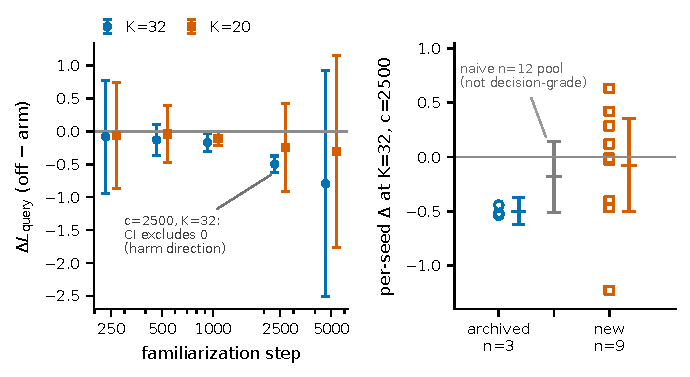
\includegraphics[width=0.92\linewidth]{figures/fig3_transient_replication.pdf}
\caption{The transient and its stopped replication. Left: per-checkpoint
arm effect $\Delta L_q$ (control minus per-token arm, encyclopedic corpus)
with three-seed 95-percent intervals at both loads; the single reading
satisfying the registered differential condition is at checkpoint 2{,}500,
$K{=}32$ ($-0.500$, $[-0.624,-0.376]$), in the harm direction, against a
non-determinate $K{=}20$ reading at the same checkpoint (mean $-0.252$,
$[-0.920,+0.416]$), and dissolves by checkpoint 5{,}000 (mean $-0.795$,
$[-2.513,+0.923]$). Right: the same anchor cell at $n{=}12$; the archived
three-seed cohort (circles, interval $[-0.624,-0.376]$) and the new
nine-seed cohort (squares, interval $[-0.506,+0.357]$) fail the
pre-registered variance-ratio gate (4.47 against a pre-registered
heuristic cutoff of 4.0; a calibrated one-sided 5-percent $F(2,8)$ test
would itself require $\approx 4.46$), so the naive pooled interval (gray,
dotted) is diagnostic only and no decision-grade pooled verdict exists.}
% evidence: C6-transient, C7-replication
\label{fig:transient}
\end{figure}

\section{Reproducibility}
\label{app:repro}

Every number in this paper is computed from archived raw result files
(per-cell JSON records written by the experiment chains at run time), not
from summaries. All figures regenerate from one versioned script that
loads only those archived files and asserts the md5 checksum of every file
it reads against a recorded manifest, so a changed or substituted artifact
fails the build rather than silently altering a panel. As a compute
disclosure for this venue's small-scale remit: all experiments ran on one
or two GPUs at a time, and the six waves consumed approximately 9.5
GPU-hours in total. % evidence: C9-compute
The archived raw files, the figure script with its checksum manifest, the
experiment chains, and the full pre-registration text will be released
with the camera-ready version.

\end{document}
